\documentclass[12pt]{article}
\usepackage[spanish]{babel}
\usepackage{makeidx}
\usepackage[margin=1in]{geometry}  % set the margins to 1in on all sides
\usepackage{graphicx}              % to include figures
\usepackage{amsmath}               % great math stuff
\usepackage{amsfonts}              % for blackboard bold, etc
\usepackage{amsthm}                % better theorem environments
\usepackage{makeidx}               % index
\usepackage[utf8]{inputenc}        % now we have tildes!
\usepackage{wrapfig}               % images
\usepackage{listings}              % Unordered lists
\usepackage{hyperref}              % hyperlinks
\usepackage{xcolor}                % to colorize font
\usepackage{blindtext}             % to colorize font
\usepackage{caption}
\usepackage{subcaption}

\makeindex

\begin{document}

\begin{titlepage}

\newcommand{\HRule}{\rule{\linewidth}{0.5mm}} % Defines a new command for the horizontal lines, change thickness here

\center % Center everything on the page

%----------------------------------------------------------------------------------------
%   LOGO SECTION
%----------------------------------------------------------------------------------------

\textsc{\LARGE Universidad Carlos III de Madrid}\\[1.2cm] % Name of your university/college

%----------------------------------------------------------------------------------------
%   HEADING SECTIONS
%----------------------------------------------------------------------------------------


\includegraphics[width=9cm]{Logo}\\[1.2cm] % Include a department/university logo - this will require the graphicx package

\textsc{\Large Aprendizaje Automático}\\[0.5cm] % Major heading such as course name
\textsc{\large Grado en Ingeniería Informática}\\[0.6cm] % Minor heading such as course title
\textsc{\large Grupo 83}\\[0.5cm]

%----------------------------------------------------------------------------------------
%   TITLE SECTION
%----------------------------------------------------------------------------------------

\HRule \\[0.7cm]
{ \huge \bfseries Práctica 3: Aprendizaje por refuerzo}\\[0.4cm] % Title of your document
\HRule \\[0.7cm]

%----------------------------------------------------------------------------------------
%   AUTHOR SECTION
%----------------------------------------------------------------------------------------

\textit{Autores:}\\
Daniel \textsc{Medina García}\\ % Your name
Alejandro \textsc{rodríguez Salamanca}\\[1.1cm] % Your name

%----------------------------------------------------------------------------------------
%   DATE SECTION
%----------------------------------------------------------------------------------------

{\large \today}\\ % Date, change the \today to a set date if you want to be precise

%----------------------------------------------------------------------------------------

\vfill % Fill the rest of the page with whitespace

\end{titlepage}

\tableofcontents

\newpage
\thispagestyle{empty}
\clearpage
\vspace*{\fill}
\begin{center}
    \begin{minipage}{\textwidth}
        \begin{center}
            \section*{Introducción}

            % TODO

        \end{center}
    \end{minipage}
\end{center}
\vfill

\newpage

\section{Diagrama con los diferentes pasos de la tarea de aprendizaje realizada en la práctica}
% TODO: Ni puta idea de esto, pero viene en el guión. Entiendo que será algo como diseñar el espacio de estados - programar el agente - aprendizaje online - generar el agente final

\section{Generación del espacio de estados}

% Hablar de nuestro estado (dirección en la que se encuentra el fantasma más cercano y última direccion en la que se ha movido Pacman).
% Justificación del conjunto de atributos final elegido y su rango para la definicion de los estados. Se debe indicar la evolucion historica de los agentes implementados hasta llegar al agente final, donde cada uno de estos agentes puede tener un conjunto de atributos diferente y destacar las diferencias con el conjunto final.
%
% Alternativas para el espacio de estados:
% \begin{enumerate}
%     \item Dirección del fantasma más cercano, si hay muros alrededor.
%     \item El usado (y que ha perdido) Dani
%     \item Dirección del fantasma mas cercano y última dirección en la que se ha movido Pacman
% \end{enumerate}

% TODO: Intro de la sección

Primero, probamos un espacio de estados formado por la dirección en la que se encuentra el fantasma más cercano, y si existen muros alrededor de PacMan, esto es, si el fantasma más cercano se encuentra por encima de PacMan y a la izquierda de éste, y hay un muro justo debajo, el estado sería \texttt{North,West,False,False,True,False}. Este espacio de estados nos daba un total de 256 estados (cuatro posibles valores de los dos primeros atributos, y dos posibles valores de los cuatro siguientes).
Tras ejecutar un agente con este espacio de estados, nos dimos cuenta de que la información relativa a los muros no aportaba información relevante puesto que en nuestro agente sólo elegimos una acción de entre las legales, y aquellas direcciones en las que se encuentra un muro no están incluídas en dicho conjunto.

Después, probamos a eliminar dicha información sobrante y nos quedamos con un conjunto de estados compuesto por
% TODO: DANI, AQUÍ TE TOCA EXPLICAR EL QUE HAS ELEGIDO TÚ.

Finalmente, el conjunto de estados elegido fue el formado por la dirección del fantasma más cercano y la dirección del último movimiento realizado por PacMan. Esto nos da un total de 64 posibles estados. Estos atributos fueron elegidos por dos razones:
\begin{itemize}
	\item Simplifica mucho el conjunto de estados — Al tener en cuenta únicamente tres atributos, el conjunto de estados queda muy reducido, lo que era uno de los objetivos que tratábamos de cumplir, puesto que un conjunto de estados muy grande puede contener estados que no se lleguen a alcanzar nunca.
	\item Aporta información necesaria y genérica — Otro de los requisitos que hemos intentado cumplir ha sido obtener un agente genérico que no esté \textit{atado} a ningún mapa, y que sea capaz de desenvolverse con soltura en diversos escenarios. Por ello, los atributos escogidos son independientes del mapa, pero aportan la información que necesita PacMan para determinar hacia qué dirección debe moverse.
\end{itemize}

\section{Generación de la \textit{tabla Q}}

Para generar la \textit{tabla Q} hemos hecho uso de la técnica conocida como \textit{online learning}. Se trata de un método mediante el cual los datos se encuentran disponibles en orden secuencial (se generan mientras PacMan está jugando partidas) y son usados para actualizar la mejor predicción hasta el momento de la \textit{tabla Q} dado un estado y una acción.

En cuanto a los refuerzos, hemos decidido dividirlos en tres tipos:
\begin{itemize}
	\item \textbf{PacMan se come un fantasma}. Cuando PacMan se come un fantasma, recibe un refuerzo positivo con un valor de 199, coincidiendo con la diferencia de puntuación entre el estado actual y el próximo estado al que se transiciona.
	\item \textbf{PacMan se acerca al fantasma más cercano}. En este caso, entendemos que PacMan está realizando un movimiento beneficioso, por el cual recibe un refuerzo positivo con valor 10.
	\item \textbf{PacMan se aleja del fantasma más cercano}. Si PacMan está \textit{persiguiendo} a un fantasma y su distancia a éste aumenta, se penaliza el movimiento con un refuerzo negativo con valor -1.
\end{itemize}

Tras probar diversas maneras de dar refuerzo a nuestro agente, la descrita previamente es la que mejor funcionó y la que se adaptaba mejor cuando variábamos el tipo de mapa. Pese ello, en un principio los refuerzos intermedios no dieron un resultado tan bueno como esperábamos; si se está jugando en un mapa con muros que no permiten a PacMan tomar el camino más directo hacia su presa, el acercarse al fantasma no siempre indica avanzar en la dirección correcta pero siempre genera refuerzo positivo.

Además, se ha usado la técnica $\epsilon$-greedy, por la cual nuestro agente toma la acción devuelta por la política obtenida hasta el momento un $\epsilon$\% de las veces, y (1-$\epsilon$)\% una acción aleatoria, para que el mapa sea explorado y se prueben diversas acciones para un mismo estado, con el objetivo de quedarnos con la que se considere mejor.

\section{Construcción del gente automático}

Nuestro agente ha sido implementado sobre la clase \texttt{PacmanQAgent}, la cual extiende de \texttt{QLearningAgent}, por lo que trae cierto comportamiento predefinido para que resulte más sencillo implementar un agente utilizando la técnica de Q-Learning.

Para ello, primero se inicializan los valores de \texttt{alpha, epsilon} y \texttt{discount} en el constructor de la clase, para ser usados posteriormente en la actualización del valor en la \textit{tabla Q}. Además, se carga la \textit{tabla Q}, que se encuentra en un fichero llamado \texttt{qtable.txt}. Esta \textit{tabla Q} es almacenada en un objeto de tipo \texttt{Counter}, que se encuentra en \texttt{utils.py}. Dicho objeto actúa como un diccionario, en el que las claves serán tuplas estado-acción, y el valor, el correspondiente al que retorne la función Q.

Nuestra política es retornada por el método \texttt{getPolicy}. Este método recibe un estado, e itera sobre todas las acciones legales, devolviendo aquella acción cuyo valor en la tabla es el máximo para el estado dado.

Si una partida supera los 800 turnos, ésta acaba, pues entendemos que nuestra tabla no se está actualizando con valores que ayuden a nuestro agente a jugar mejor.

Finalmente, al final de cada turno, el método \texttt{update} es llamado. Este método recibe como parámetros el estado actual, el estado al que se transiciona, la acción realizada y el refuerzo obtenido con dicha acción. Aquí es donde se encuentra implementada la función de actualización:

\begin{equation*}
	Q(s,a)\gets(1-\alpha) Q(s,a)+\alpha [r+\gamma max_a (s,a)]
\end{equation*}

\newpage
\section{Evaluación}
Para nuestro agente, hemos decidido probar dos configuraciones distintas a partir de las cuales hemos generados dos \textit{tablas Q} que nos dispondremos a evaluar.

\begin{figure}[h]
    \centering
    \begin{subfigure}{.5\textwidth}
        \centering
        \begin{tabular}{ l | c}
        	\hline
        	$\alpha$	& 0.3 \\ \hline
        	$\gamma$	& 0.8 \\ \hline
        	$\epsilon$	& 0.8 \\
        	\hline
        \end{tabular}
        \caption{Agente 1}
        \label{fig:sub1}
    \end{subfigure}%
    \begin{subfigure}{.5\textwidth}
        \centering
        \begin{tabular}{ l | c}
        	\hline
        	$\alpha$	& 0.6 \\ \hline
        	$\gamma$	& 0.4 \\ \hline
        	$\epsilon$	& 0.7 \\
        	\hline
        \end{tabular}
        \caption{Agente 2}
        \label{fig:sub2}
    \end{subfigure}
\end{figure}

Para realizar la evaluación de ambas configuraciones hemos jugado 10 partidas en el mapa por defecto y en \texttt{finalMap} para comprobar cómo se comportaba el agente en dos escenarios completamente diferentes. Primero, evaluamos los datos obtenidos con los parámetros previamente mostrados, obteniendo los resultados que muestra la figura a continuación.

\begin{figure}[h]
    \centering
    \begin{subfigure}{.5\textwidth}
        \centering
        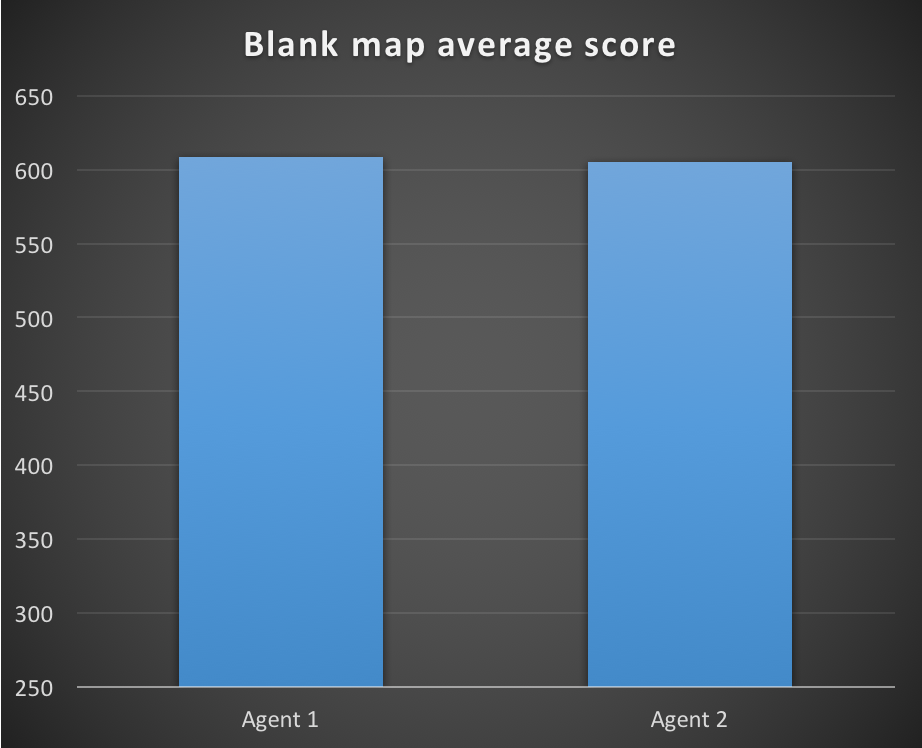
\includegraphics[width=.7\linewidth]{bmap_a}
        \caption{Default map}
        \label{fig:sub1}
    \end{subfigure}%
    \begin{subfigure}{.5\textwidth}
        \centering
        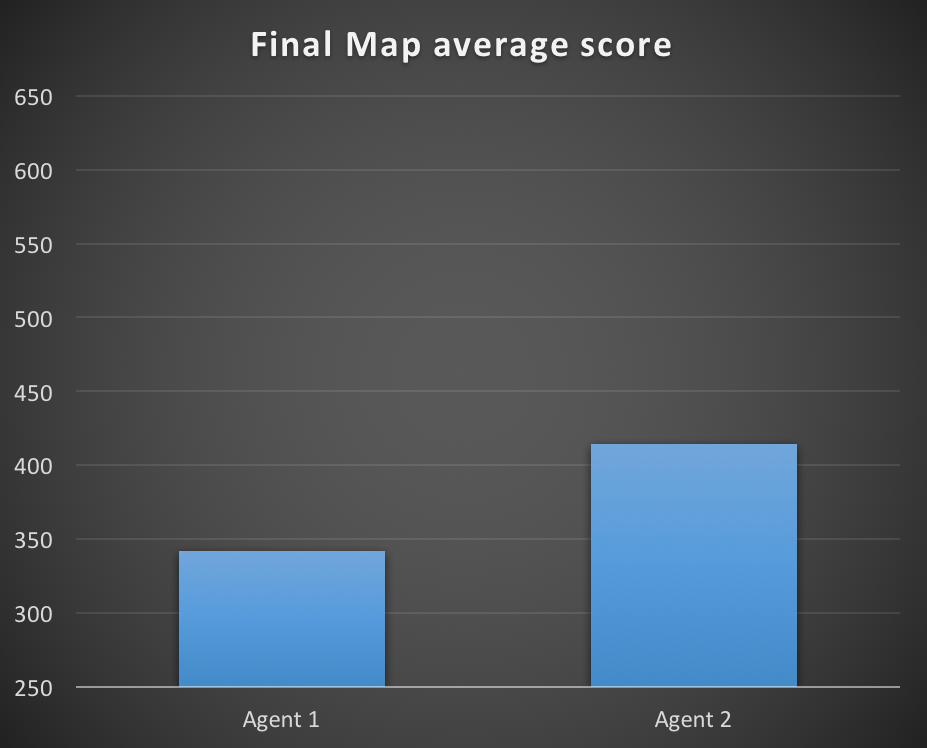
\includegraphics[width=.7\linewidth]{fmap_a}
        \caption{Final map}
        \label{fig:sub2}
    \end{subfigure}
    \caption{Rendimiento por agentes durante el aprendizaje}
    \label{fig:test}
\end{figure}

Más tarde, utilizaremos siempre la acción que indique nuestra política, sin actualizar los valores de la \textit{tabla Q} durante las distintas partidas para observar las diferencias. La siguiente figura muestra estos resultados para el mapa por defecto.

\begin{figure}[h]
    \centering
    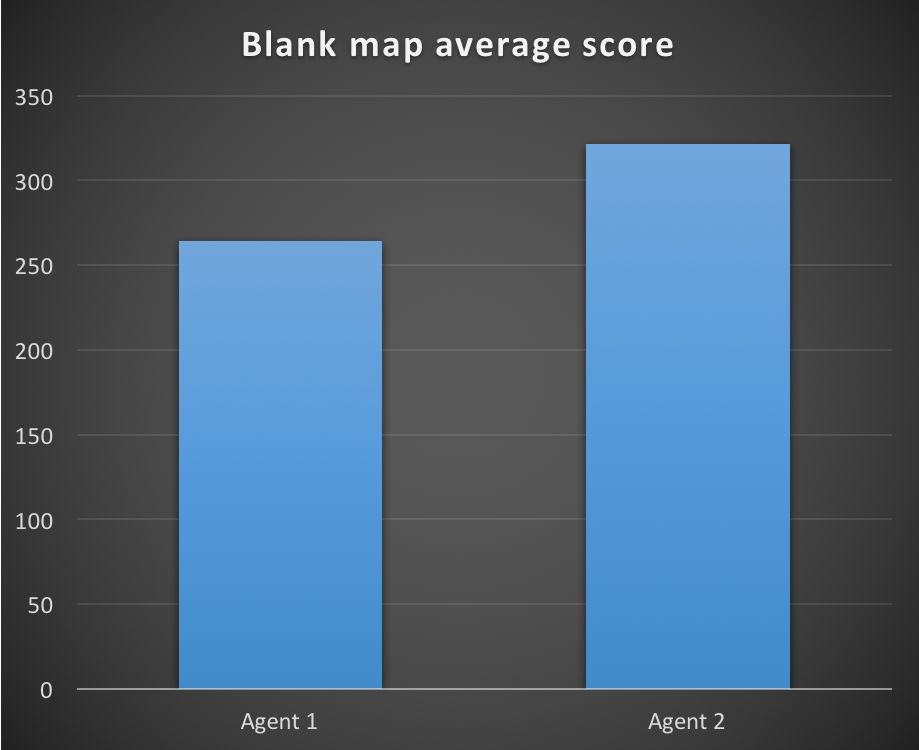
\includegraphics[width=6cm]{bmap_b}
    \caption{Rendimiento por agentes siguiendo únicamente la política}
\end{figure}

\newpage
Pese a la mayor media de puntuación observada aquí en el segundo agente, cabe destacar la ausencia de \textit{timeouts} en el primer agente, mientras que el agente 2 abandonó un 30\% de las partidas jugadas. Un \textit{timeout} se produce cuando la partida sobrepasa los 2000 turnos, habitualmente causado por la entrada en un bucle.
También indicar que la ausencia de datos para el \textit{Final map} se debe que todas las partidas acabaron en \textit{timeout} para ambos agentes.

\vspace{0.5cm}

Como podemos observar, en aquellas partidas jugadas con un porcentaje de movimientos aleatorios y en las cuales la \textit{tabla Q} se actualiza, obtenemos unos resultados mucho mejores que cuando seguimos siempre la acción que devuelve nuestra política y mantenemos la \textit{tabla Q} invariable. Esto puede ser debido a:

\begin{itemize}
	\item \textbf{Nuestro agente no ha aprendido aún la política óptima} - Pese a haber jugado un elevado número de partidas con nuestro agente para conseguir una \textit{tabla Q} fiable cuyos valores se correspondiesen con la acción más adecuada para cada instante, no hemos conseguido que el algoritmo obtenga los valores adecuados, o la forma en la que expresamos los estados no es la más adecuada.
	\item \textbf{La definición de estado que usamos es muy general} - Al intentar usar una definición de estado lo más genérica posible y haber entrenado en diversos mapas, existe la posibilidad de que nuestro agente no sepa desenvolverse con soltura en ninguno.
\end{itemize}

Tras valorar los resultados, hemos llegado a la conclusión de que la gran diferencia obtenida es debido al segundo caso, puesto que cuando el agente realiza ciertas acciones aleatorias que le ayudan a explorar un mapa y salir de aquellas situaciones en las que no tiene claro qué debe hacer, y es capaz de actualizar la \textit{tabla Q} para \texttt{recordar} esas decisiones en futuras partidas, es capaz de obtener unas puntuaciones muy buenas en las partidas jugadas, y más teniendo en cuenta los datos con los que cuenta para tomar las decisiones.

\vspace{0.5cm}

Dada la inestabilidad del segundo agente y el parecido rendimiento de ambos cuando los dos funcionan con normalidad, elegimos el primer agente como el final para nuestro equipo.

\section{Agente final}

% TODO: (con el que mejores resultados obtenga de lo anterior)

% Descripción y análisis de los resultados producidos por el agente final implementado tras la evaluación. En este apartado es importante describir por que se cree que ha funcionado bien el agente seleccionado (si es este el caso). En cualquier caso, se deberán describir posibles mejoras que se pueden hacer para aumentar su rendimiento. Ademas, es importante responder a la siguiente cuestion:
% ¿El agente final desarrollado es capaz de superar en rendimiento a los agentes utilizados en la generacion de las tuplas de experiencia? Justificar la respuesta tanto en caso afirmativo como en caso contrario.


\section{Conclusiones}
% TODO: Conclusiones sobre la tarea a realizar.
% Apreciaciones mas generales sobre las practicas de la asignatura como: para que pueden ser utiles los modelos obtenidos y si se os ocurren otros dominios en los que aplicar aprendizaje automatico, etc.
% Descripcion de los problemas encontrados a la hora de realizar esta practica.
% Comentarios personales. Opinion acerca de la practica. Dificultades encontradas, criticas, etc
\end{document}
